\documentclass[11pt,a4paper]{article}
\usepackage[margin=23mm]{geometry}
\usepackage[T1]{fontenc}
\usepackage{lmodern,microtype,amsmath,amssymb,graphicx,booktabs}
\usepackage[hidelinks]{hyperref}
\setlength{\parindent}{0pt}
\setlength{\parskip}{5pt}
\setlength{\emergencystretch}{2em}
\newcommand{\MonoError}{5.684\times10^{-14}}
\newcommand{\TangentError}{9.093\times10^{-11}}
\newcommand{\BalanceError}{8.704\times10^{-14}}
\newcommand{\BarError}{1.364\times10^{-12}}
\newcommand{\NodalError}{3.331\times10^{-16}}
\newcommand{\Stored}{1.639064}
\newcommand{\Dissipated}{9.287179}
\newcommand{\Work}{10.960207}
\newcommand{\Defect}{0.033964}
\newcommand{\Order}{0.998363}
\newcommand{\BarStress}{232.142857}

\title{YieldLedger: separating plastic dissipation\newline from endpoint-work error}
\author{Computational mechanics project report}
\date{30 September 2026}
\begin{document}
\maketitle
\begin{abstract}
An energy balance can close while its interpretation remains wrong: in incremental
plasticity, endpoint force--displacement work includes a nonnegative quadrature
excess that is distinct from irreversible material dissipation. This report studies
that distinction in a small-strain uniaxial mixed-hardening model. An original C++
return-mapping kernel is coupled to a Python bar finite-element solver with committed
material history and a safeguarded Newton iteration. Synthetic cyclic and analytical
bar experiments verify yield admissibility, consistent tangents and a discrete energy
identity. The final work-excess refinement order is $\Order$. For a two-element
bar, consistent and elastic tangents require one and 72 corrections, respectively.
These results verify a specified numerical model; they do not validate a physical
material or establish a general solver speedup.
\end{abstract}

\section{Question, assumptions and constitutive model}
The research question is whether plastic dissipation can be reported independently
of load-increment work error while preserving a reliable global equilibrium solve.
Return mapping and consistent tangents are standard tools in computational
plasticity~\cite{bleyer}; mixed hardening provides both a translating and expanding
yield interval~\cite{moose}. Here their simplest one-dimensional linear form makes
the energy accounting and reference solutions transparent. No new constitutive law
or return-mapping algorithm is claimed.

Consider a bar with constant area $A$, no body force, imposed end displacements
$u(0)=0$, $u(L)=U$, and infinitesimal axial strain $\varepsilon=u'$. Quasistatic
equilibrium is $(A\sigma)'=0$. The internal variables are signed plastic strain $p$
and accumulated plastic strain $\alpha\geq |p|$. With positive elastic modulus $E$
and initial yield stress $\sigma_y$, and nonnegative hardening moduli $H_i,H_k$,
\begin{align}
 \sigma &= E(\varepsilon-p), &
 f &= |\sigma-H_kp|-(\sigma_y+H_i\alpha)\leq0,\label{eq:yield}\\
 \mathrm{d}p &= s\,\mathrm{d}\gamma, &
 \mathrm{d}\alpha &=\mathrm{d}\gamma\geq0,\quad f\,\mathrm{d}\gamma=0,
 \quad s=\operatorname{sign}(\sigma-H_kp).\label{eq:flow}
\end{align}
The model is rate-independent and isothermal. Hardening contributions are stored
in the chosen free-energy function, not counted as irreversible dissipation.
Stored isotropic hardening energy is not recovered by elastic unloading because
$\alpha$ cannot decrease. This constitutive assumption is not inferred from tests.

\newpage
\section{Incremental algorithm and energy identity}
At each material point, the old state $(p_n,\alpha_n)$ is held fixed during the
global solve. Given trial strain $\varepsilon_{n+1}$, define
\begin{align}
 \sigma^{\mathrm{tr}}&=E(\varepsilon_{n+1}-p_n),\qquad
 \xi^{\mathrm{tr}}=\sigma^{\mathrm{tr}}-H_kp_n,\\
 f^{\mathrm{tr}}&=|\xi^{\mathrm{tr}}|-\sigma_y-H_i\alpha_n,\qquad
 \Delta\gamma=\frac{\max(0,f^{\mathrm{tr}})}{E+H_i+H_k}.\label{eq:return}
\end{align}
Set $s=\operatorname{sign}(\xi^{\mathrm{tr}})$, $p_{n+1}=p_n+s\Delta\gamma$,
$\alpha_{n+1}=\alpha_n+\Delta\gamma$, and
$\sigma_{n+1}=\sigma^{\mathrm{tr}}-Es\Delta\gamma$. The algorithmic tangent is $E$
on the elastic branch and $E(H_i+H_k)/(E+H_i+H_k)$ on the plastic branch. At the
yield kink the code selects the elastic one-sided tangent; finite-difference
derivative checks deliberately avoid that point.

With $e=\varepsilon-p$, the stored energy and incremental irreversible dissipation are
\begin{equation}
 \psi=\tfrac12Ee^2+\tfrac12H_i\alpha^2+\tfrac12H_kp^2,
 \qquad \Delta D=\sigma_y\Delta\alpha.\label{eq:energy}
\end{equation}
Using $x_{n+1}\Delta x=\Delta(x^2)/2+(\Delta x)^2/2$ and the return condition gives
\begin{align}
 \sigma_{n+1}\Delta\varepsilon&=\Delta\psi+\Delta D+Q,\label{eq:identity}\\
 Q&=\tfrac12 E(\Delta e)^2+\tfrac12H_i(\Delta\alpha)^2+
       \tfrac12H_k(\Delta p)^2\geq0.\label{eq:defect}
\end{align}
In plastic loading, $\sigma_{n+1}\Delta p=(\sigma_y+H_i\alpha_{n+1})\Delta\alpha+
H_kp_{n+1}\Delta p$; in elasticity both plastic increments vanish. Thus the identity
also holds for steps that cross yield. Summing it separates endpoint work, stored
energy, irreversible dissipation and $Q$ without an inferred residual category.

\subsection{Implementation and global solution}
The C++17 header implements the closed-form update, finite-input/state checks and
stored energy. pybind11 exposes read-only material, state and response objects.
Python assembles P1 bar elements with one constant-strain point each:
$\mathbf f_e=A\sigma_e[-1,1]^T$ and
$\mathbf K_e=AC_e\left[\begin{smallmatrix}1&-1\\-1&1\end{smallmatrix}\right]/\ell_e$.
The free-node residual is solved with dense linear algebra. A correction is halved
up to 29 times until the infinity-norm residual decreases by an Armijo factor
$10^{-4}$ or meets the final force tolerance. Each trial starts from the same old
material state. Only convergence commits history; failed solves raise an exception.
Positive total hardening is required by the bar API to exclude fully plastic singular
tangents. The point kernel separately supports perfect plasticity.

\subsection{Reproducible experiment definitions}
Material-point stresses use MPa: $E=200000$, $\sigma_y=250$, $H_i=2000$, $H_k=3000$.
Strain visits zero, 0.008, $-0.008$, 0.008, and zero, with $N$ equal increments
per leg, $N=25,50,100,200,400,800$. Every reversal is sampled; $N=400$ is the main
record. A 501-point monotonic path from zero to 0.02 is compared with the exact
bilinear law. Four tangent checks use central differences of size $10^{-8}$ after
preloading to 0.004. Their error is normalized by $E$.

\newpage
\section{Measured validation results}
The bar has $A=10\,\mathrm{mm}^2$, layer lengths $(40,60)$ mm, elastic moduli
$(200000,100000)$ MPa, yield stresses $(200,400)$ MPa, and total hardening moduli
$(6000,10000)$ MPa. Their $(H_i,H_k)$ splits are $(2000,4000)$ and $(5000,5000)$.
At $U=0.4$ mm, only the first layer is plastic. Equilibrium and compatibility give
\begin{equation}
 \sigma_* = \frac{U+L_1\sigma_{y1}/H_1}
 {L_1/E_1+L_2/E_2+L_1/H_1}=\BarStress\ \mathrm{MPa}.\label{eq:bar}
\end{equation}
Meshes split each layer into 1, 4 or 16 elements. Newton stopping uses absolute
tolerance $10^{-10}$ N plus $10^{-10}\max(1,\max_e|A\sigma_e|)$ N. The iteration
comparison starts from a virgin two-element bar and an affine displacement guess.

\begin{figure}[ht]
 \centering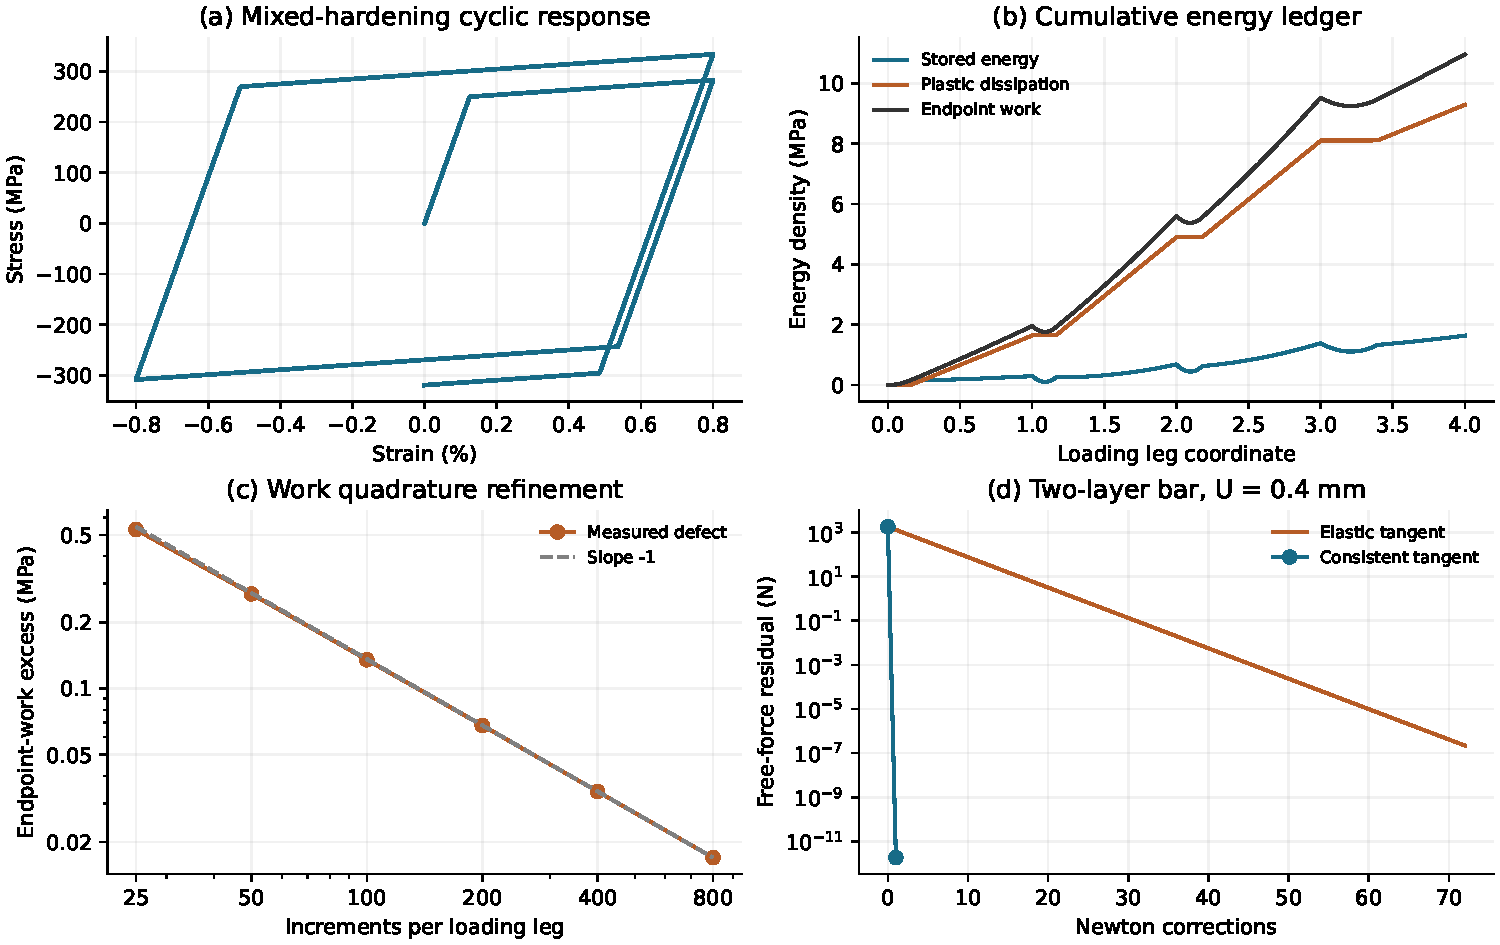
\includegraphics[width=\linewidth]{../results/overview.pdf}
 \caption{Original recorded experiments: cyclic stress response; cumulative energy
 components; endpoint-work excess under refinement; and the two-element bar residual.
 The last panel compares corrections, not execution time.}
 \label{fig:results}
\end{figure}

\begin{table}[ht]
\centering\small
\begin{tabular}{@{}lr@{}}
\toprule
Verification quantity & Recorded value\\\midrule
Maximum monotonic stress error (MPa) & $\MonoError$\\
Maximum tangent error divided by $E$ & $\TangentError$\\
Maximum cumulative energy-identity error (MPa) & $\BalanceError$\\
Maximum aligned-bar stress error, all meshes (MPa) & $\BarError$\\
Maximum aligned-bar nodal error, all meshes (mm) & $\NodalError$\\
Consistent / elastic tangent corrections, two elements & $1\,/\,72$\\
\bottomrule
\end{tabular}
\caption{Deterministic verification values from the committed numerical outputs.
Near-roundoff errors are platform dependent, not attainable accuracy guarantees.}
\label{tab:errors}
\end{table}

\newpage
\section{Discussion: what the errors do and do not measure}
For the main 1,600-increment path, final stored energy is $\Stored$ MPa,
irreversible dissipation is $\Dissipated$ MPa, endpoint work is $\Work$ MPa,
and endpoint-work excess is $\Defect$ MPa. Here MPa is an energy density
($\mathrm{N\,mm}/\mathrm{mm}^3$). The final strain is zero but internal variables
and residual stress need not vanish. Consequently this is not a closed state-space
cycle and its total work must not be equated with plastic dissipation alone.

For this one-dimensional law, return mapping gives exact endpoint states along
each monotonic imposed-strain leg, including a yield transition. Continuum work
on the resolved path is the change in stored energy plus $\sigma_y\Delta\alpha$.
Thus $Q$ is a work-quadrature error, not an added physical mechanism. Its measured
order approaches one: the final pair of refinements gives $\Order$. This observation
does not establish first-order error for every internal variable or every loading
path. Reversals absent from the sampled path cannot be reconstructed by this method.

The aligned bar has piecewise constant strain and piecewise affine displacement.
The exact continuum solution therefore lies in every tested P1 space. Table
\ref{tab:errors} primarily measures nonlinear algebraic and floating-point error,
not a spatial convergence rate. No general claim is made about curved geometries,
non-aligned interfaces, heterogeneous elements, or multiaxial finite elements.
The one-versus-72 comparison demonstrates the value of the consistent derivative
for this particular equilibrium problem. It does not measure runtime, account for
all trial evaluations, or prove global Newton convergence. Backtracking was needed
to prevent active-set cycling in refined meshes whose initial guesses lay at yield.

\section{Reproducibility, limits and conclusion}
The repository includes 39 Python tests and a native 2,000-update cyclic invariant
test covering analytical response, reverse yield, complementarity, tangents, energy,
equilibrium and failed-step state preservation. Run \texttt{yieldledger --output results}
and \texttt{python paper/build.py --engine pdflatex} from an installed checkout.
The builder derives numerical macros from recorded metrics, hashes inputs, checks
references and layout, and enforces a five-page limit. CSV data and CI are included.

No physical calibration is provided. Finite strains, thermal effects, viscosity,
damage, multiaxial response and fatigue are excluded. Unsaturated linear hardening
is an idealization. Dense matrices, no automatic step cutback, and bounded
backtracking limit scale and robustness. Numerical verification does not establish
physical validity or suitability for design.

Within these limits, the explicit ledger separates dissipation from endpoint-work
excess, while committed-state updates and consistent tangents produce a verifiable
equilibrium solution. Separate reporting makes refinement results interpretable.

\begin{thebibliography}{9}\small
\bibitem{bleyer} J. Bleyer et al., \emph{Elasto-plastic analysis of a 2D von Mises material},
Computational Mechanics Numerical Tours with FEniCSx. Public numerical-method background.
\url{https://bleyerj.github.io/comet-fenicsx/tours/nonlinear_problems/plasticity/plasticity.html}.
Accessed 30 September 2026.
\bibitem{moose} MOOSE, \emph{Combined Nonlinear Hardening Plasticity}, public framework
documentation. Describes broader nonlinear hardening models than used here.
\url{https://mooseframework.inl.gov/moose/source/materials/CombinedNonlinearHardeningPlasticity.html}.
Accessed 30 September 2026.
\end{thebibliography}
\end{document}
